\section{3. Problem 2}
\vspace{10pt}

\subsection{3.1 USE CASE DIAGRAM}
\vspace{10pt}
\begin{figure}[H]
	\centering
	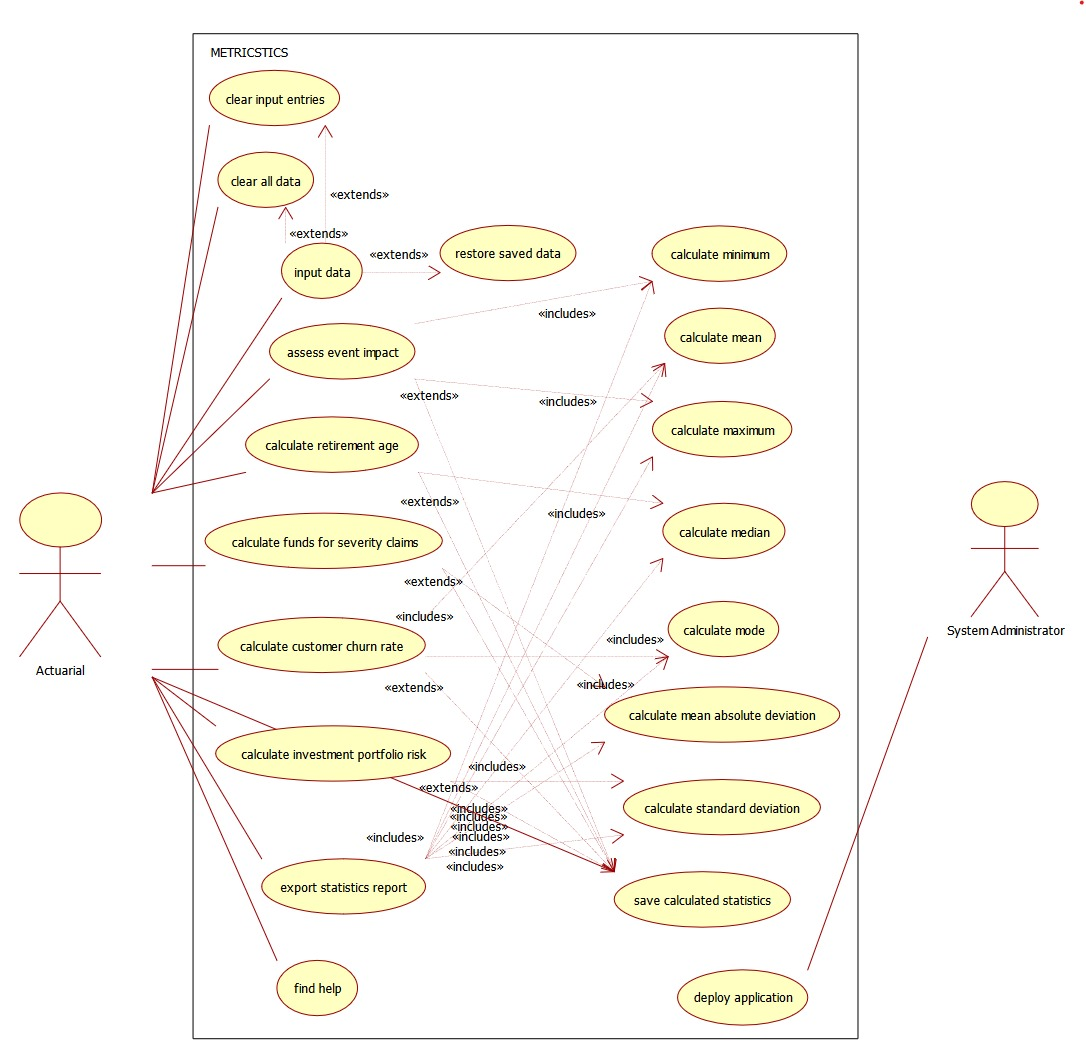
\includegraphics[width=\linewidth,height=15cm]{d1/UseCase Team R.jpeg}
	\caption{Use Case Diagram} 
	\label{CRC}
\end{figure}
\vspace{100pt}
\subsection{3.2 USE CASES}
\subsubsection{Actors}
\hspace{0.5cm}\textbf {Actuarial}\\

The main user of the METRICSTICS system is Actuarial. The primary work of Actuarial is to assess financial risks in the insurance and finance fields, using mathematical and statistical methods.\\

\textbf{System Administrator}\\

The secondary user of the METRICSTICS system is System Administrator. The primary work of System Administrator is to deploy and maintain the METRICSTICS System.\\

% \begin{table}
%     \centering
%     \begin{tabular}{|c|c|c|} \hline 
%          No&  Question& Metric(s)\\ \hline 
%          1&  aaa sss sssss sss dsds ds dsadasd ad dasdasd& \\ \hline 
%          2&  & \\ \hline 
%          3&  & \\ \hline 
%          4&  & \\ \hline 
%          5&  & \\ \hline 
%          6&  & \\ \hline 
%          7&  & \\ \hline 
%          8&  & \\ \hline 
%          9&  & \\ \hline 
%  10& &\\ \hline
%     \end{tabular}
%     \caption{Question - Metrics table}
%     \label{tab:my_label}
% \end{table}





\begin{table}[htb]
    \centering
    \begin{tabular}{|p{4cm}|p{12cm}|} \hline 
         System &  METRICSTICS\\ \hline 
         
         Identifier & UC-001 \\ \hline 
         
         \multirow{2}{*}{Author} & Manasa Yalakala  \\
         &manasayalakala@gmail.com \\
           \hline 
           Version & 1.0\\ \hline
         
         Priority &  Medium\\ \hline 
         
         Name & Find Help \\ \hline 
         Pre-conditions & The system is running and accessible. \\ \hline 
         Post-conditions &  The system displays the help documentation. \\ \hline
         Trigger & The actuarial clicks the help button on the system interface. \\ \hline
        \multirow{2}{*}{Normal flow} 
        & \textbf{1.} The actuarial clicks the help button. \\ 
        & \textbf{2.} The the system displays the help documentation. \\  
        
        \hline
         \multirow{2}{*}{Exceptional flow} 
        & \textbf{1.} The help documentation fails to load. \\ 
        & \textbf{2.} The system displays an error. \\ 
        \hline
         Related actors & Actuarial  \\ \hline
        Related use case & None \\ \hline
         
    \end{tabular}
    \caption{Use Case Description for Find Help}
    \label{tab:my_label}
\end{table}
\begin{table}[htb]
    \centering
    \begin{tabular}{|p{4cm}|p{12cm}|} \hline 
         System &  METRICSTICS\\ \hline 
         
         Identifier & UC-002 \\ \hline 
         
         \multirow{2}{*}{Author} & Manasa Yalakala  \\
         &manasayalakala@gmail.com \\
           \hline 
         Version & 1.0\\ \hline
         Priority &  Medium\\ \hline 
         
         Name & Clear  All Data. \\ \hline 
         Pre-conditions & User is logged into the METRICSTICS system. \\ \hline 
         Post-conditions & Data in the system is cleared as requested by the actuarial. \\ \hline
         Trigger & The actuarial selects the option to clear all data from the METRICSTICS system. \\ \hline
        \multirow{4}{*}{Normal flow} 
        & \textbf{1.}  The system presents the actuarial with an option to confirm data clearance. \\ 
        & \textbf{2.} The actuarial confirms the data clearance request. \\ 
        & \textbf{3.} The system deletes all data stored in METRICSTICS, including input datasets and calculation results. \\ 
        & \textbf{4.} The system displays a confirmation message to the actuarial, indicating that the data has been successfully cleared. \\ 
         
        
        \hline
        \multirow{2}{*}{Exceptional flow} 
        & \textbf{1.}  If the actuarial cancels the data clearance request, the system returns to the main menu without clearing any data. \\ 
        & \textbf{2.}  If there is a technical issue preventing data clearance, the system displays an error message and logs the issue for technical support. \\  \hline 
        Related actors & Actuarial \\ \hline
        Related use case & None  \\ \hline
    \end{tabular}
    \caption{Use Case Description for Clear All Data}
    \label{tab:my_label}
\end{table}
\begin{table}[htb]
    \centering
    \begin{tabular}{|p{4cm}|p{12cm}|} \hline 
         System &  METRICSTICS\\ \hline 
         
         Identifier & UC-003 \\ \hline 
         
         \multirow{2}{*}{Author} & Neha Velagapudi  \\
         &nehavelagapudi07@gmail.com \\
           \hline 
           Version & 1.0\\ \hline
         
         Priority &  Medium\\ \hline 
         
         Name & Save Calculated Statistics. \\ \hline 
         Pre-conditions & User is logged into the METRICSTICS system, and descriptive statistics have been calculated. \\ \hline 
         Post-conditions & Calculated descriptive statistics are saved for future reference. \\ \hline
         Trigger & The user selects the option to save calculated statistics within METRICSTICS. \\ \hline
        \multirow{5}{*}{Normal flow} 
        & \textbf{1.}   The system presents the user with a list of datasets for which descriptive statistics have been calculated. \\ 
        & \textbf{2.} The user selects a dataset for which they want to save the calculated statistics. \\ 
          & \textbf{3.} The system prompts the user to provide a name or description for the saved statistics. \\ 
        & \textbf{4.} The user enters a name or description and confirms the save action. \\ 
        & \textbf{5.} The system stores the calculated statistics with the provided name/description for future retrieval. \\ 
       
         
        
        \hline
         \multirow{2}{*}{Exceptional flow} 
        & \textbf{1.}If the user attempts to save statistics for a dataset that has not had descriptive statistics calculated, the system informs the user and prompts them to perform calculations first. \\ 
        & \textbf{2.}If there is an issue with saving due to storage limitations or file system errors, the system notifies the user and suggests freeing up storage space or checking file permissions. \\  \hline 
        Related actors & Actuarial \\ \hline
        Related use case & None \\ \hline
    \end{tabular}
    \caption{Use Case Description for Save Calculated Statistics}
    \label{tab:my_label}
\end{table}
\begin{table}[htb]
    \centering
    \begin{tabular}{|p{4cm}|p{12cm}|} \hline 
         System &  METRICSTICS\\ \hline 
         
         Identifier & UC-004 \\ \hline 
         
         \multirow{2}{*}{Author} & Revanth V  \\
         &vrevanth.278@gmail.com \\
           \hline 
           Version & 1.0\\ \hline
         
         Priority &  Medium\\ \hline 
         
         Name & Restore Saved Data. \\ \hline 
         Pre-conditions & The system is running and accessible.
There are saved data for previous data input and/or calculation results.\\ \hline 
         Post-conditions & The previously saved data and/or result are restored and displayed. \\ \hline
         Trigger & The user clicks the “Restore” button. \\ \hline
        \multirow{2}{*}{Normal flow} 
        & \textbf{1.}The user clicks the “Restore” button. \\ 
        & \textbf{2.} The system retrieves saved data and display it in the interface.  \\ 
         
         \hline
         \multirow{2}{*}{Exceptional flow} 
        & \textbf{1.}There is no saved data. \\ 
        & \textbf{2.} The system displays an error.  \\  \hline 
        Related actors & Actuarial  \\ \hline
        Related use case & Input Data \\ \hline
    \end{tabular}
    \caption{Use Case Description for Restore Saved Data}
    \label{tab:my_label}
\end{table}
\begin{table}[htb]
    \centering
    \begin{tabular}{|p{4cm}|p{12cm}|} \hline 
         System &  METRICSTICS\\ \hline 
         
         Identifier & UC-005 \\ \hline 
         
         \multirow{2}{*}{Author} & Revanth V  \\
         &vrevanth.278@gmail.com\\
           \hline 
           Version & 1.0\\ \hline
         
         Priority &  Medium\\ \hline 
         
         Name &  Clear Input Entries. \\ \hline 
         Pre-conditions & The system is running and accessible.
There is data entered in the interface. \\ \hline 
         Post-conditions & The data input entries are cleared. \\ \hline
         Trigger & The user clicks the “Clear Input Entries” button.
 \\ \hline
        \multirow{2}{*}{Normal flow} 
        & \textbf{1.}  The user clicks the “Clear Input Entries” button.\\ 
        & \textbf{2.} The data input entires are cleared.\\
         
         
        
        \hline
         \multirow{2}{*}{Exceptional flow} 
        & \textbf{1.}   There is no input data or calculation results. \\ 
        & \textbf{2.} The system does nothing. \\ \hline
         Related actors & Actuarial \\ \hline
        Related use case &  Input Data\\ \hline
    \end{tabular}
    \caption{Use Case Description for Clear Input Entries}
    \label{tab:my_label}
\end{table}
\begin{table}[htb]
    \centering
    \begin{tabular}{|p{4cm}|p{12cm}|} \hline 
         System &  METRICSTICS\\ \hline 
         
         Identifier & UC-006 \\ \hline 
         
         \multirow{2}{*}{Author} & Manaswini Yarlagadda \\
         &manaswiniyarlagadda@gmail.com \\
           \hline 
           Version & 1.0\\ \hline
         
         Priority &  high\\ \hline 
         
         Name & Deploy Application \\ \hline 
         Pre-conditions & User is logged into the Deployment Manager system.
The application package is ready for deployment. \\ \hline 
         Post-conditions & The application is successfully deployed on the target environment. \\ \hline
         Trigger & The user selects the option to deploy an application from the Deployment Manager interface. \\ \hline
        \multirow{5}{*}{Normal flow} 
        & \textbf{1.} The system presents the user with a list of available applications and target environments. \\ 
        & \textbf{2.}The user selects the application to be deployed and the target environment.\\
 & \textbf{3.}  The system initiates the deployment process, including transferring application files and configuring the environment. \\ 
        & \textbf{4.}The system monitors the deployment progress and updates the user on the status.\\
 & \textbf{5.}  Once the deployment is complete, the system notifies the user of the successful deployment. \\ 
         
        
        \hline
         \multirow{2}{*}{Exceptional flow} 
        & \textbf{1.} If there are conflicts or issues during deployment, the system provides error messages and logs for troubleshooting. \\ 
        & \textbf{2.} If the selected application or target environment is unavailable, the system notifies the user and prevents deployment.\\ \hline 
        Related actors & Actuarial \\ \hline
        Related use case &  None \\ \hline
    \end{tabular}
    \caption{Use Case Description for Deploy Application}
    \label{tab:my_label}
\end{table}
\begin{table}[htb]
    \centering
    \begin{tabular}{|p{4cm}|p{12cm}|} \hline 
         System &  METRICSTICS\\ \hline 
         
         Identifier & UC-007 \\ \hline 
         
         \multirow{2}{*}{Author} & Manaswini Yarlagadda   \\
         &manaswiniyarlagadda@gmail.com \\
           \hline 
           Version & 1.0\\ \hline
         
         Priority &  Medium\\ \hline 
         
         Name & Export Statistics Report. \\ \hline 
         Pre-conditions & Mathematical Statistician is logged into the METRICSTICS system, and descriptive statistics have been calculated. \\ \hline 
         Post-conditions & A report containing descriptive statistics is exported in the user's preferred format (e.g., PDF, CSV).  \\ \hline
         Trigger & The Mathematical Statistician selects the option to export a descriptive statistics report from METRICSTICS. \\ \hline
        \multirow{6}{*}{Normal flow} 
        & \textbf{1.} The system presents the Mathematical Statistician with a list of datasets for which descriptive statistics have been calculated. \\ 
        & \textbf{2.} The Mathematical Statistician selects a dataset for which they want to export a report.   \\ 
 & \textbf{3.}  The Mathematical Statistician specifies the format (e.g., PDF, CSV) in which they want to export the report. \\ 
        & \textbf{4.}  The system generates a report containing descriptive statistics (minimum, maximum, mode, median, mean, MAD, standard deviation) for the selected dataset.   \\
 & \textbf{5.}   The system exports the report in the Mathematical Statistician's specified format. \\ 
        & \textbf{6.}  The system confirms successful export and provides a download link to the Mathematical Statistician.   \\
         
        
        \hline
        \multirow{2}{*}{Exceptional flow} 
        & \textbf{1.} If there is an issue generating or exporting the report, the system displays an error message and logs the issue for technical support. \\ 
        & \textbf{2.} If the selected dataset has not had descriptive statistics calculated, the system informs the Mathematical Statistician and prompts them to perform calculations first.   \\  \hline 
        Related actors & Actuarial \\ \hline
        Related use case & Input Data, Minimum, Maximum, Mean, Mode, Median, Standard deviation, MAD  \\ \hline
    \end{tabular}
    \caption{Use Case Description for Export Statistics Report}
    \label{tab:my_label}
   \end{table}   
\begin{table}[htb]
    \centering
    \begin{tabular}{|p{4cm}|p{12cm}|} \hline 
         System &  METRICSTICS\\ \hline 
         
         Identifier & UC-008 \\ \hline 
         
         \multirow{2}{*}{Author} & Wenxue Zhao   \\
         &wenxuezhao@gmail.com \\
           \hline 
           Version & 1.0\\ \hline
         
         Priority &  High\\ \hline 
         
         Name & Input Data. \\ \hline 
         Pre-conditions & The system is running and accessable. \\ \hline 
         Post-conditions & The system receive the dataset input from the user.  \\ \hline
         Trigger & The statistician clicked the text field to input the dataset. \\ \hline
        \multirow{3}{*}{Normal flow} 
        & \textbf{1.} The user clicks the data input text field. \\ 
        & \textbf{2.} The user enters the data.   \\ 
 & \textbf{3.}  The data is automatically saved to the browser local storage. \\ 
         
        
        \hline
        \multirow{2}{*}{Exceptional flow} 
        & \textbf{1.} The system detects the user entered invalid symbols. \\ 
        & \textbf{2.} The system displays an error message to prompt the user to enter the correct data.   \\  \hline 
        Related actors & Actuarial \\ \hline
        Related use case & Restore saved data  \\ \hline
    \end{tabular}
    \caption{Use Case Description for Input Data}
    \label{tab:my_label}
    \end{table}   
\begin{table}[htb]
    \centering
     \begin{tabular}{|p{4cm}|p{12cm}|} \hline 
         System &  METRICSTICS\\ \hline 
         
         Identifier & UC-009 \\ \hline 
         
         \multirow{2}{*}{Author} & Shashank Verma   \\
         &shashank6341@gmail.com \\
           \hline 
           Version & 1.0\\ \hline
         
         Priority &  High\\ \hline 
         
         Name & Assessment of an Event Impact. \\ \hline 
         Pre-conditions & The system is running and accessible.
Data related to catastrophic events has been successfully entered and saved by the system (as per "Input Data" use case). \\ \hline 
         Post-conditions & The minimum and maximum financial impact of catastrophic events have been calculated and displayed.  \\ \hline
         Trigger & User selects the "Calculate Minimum" option. User selects the "Calculate Maximum" option. \\ \hline
        \multirow{8}{*}{Normal flow} 
        & \textbf{1.} User selects "Calculate Minimum" from the available options. \\ 
        & \textbf{2.} The system retrieves the input data related to catastrophic events from the session.   \\ 
 & \textbf{3.} The system calculates the minimum financial impact of the catastrophic events on insurance portfolios. \\ 
 & \textbf{4.} The calculated minimum financial impact values are displayed to the user, along with relevant analysis. \\ 
        & \textbf{5.} User selects "Calculate Maximum" from the available options.  \\ 
 & \textbf{6.}  The system retrieves the input data related to catastrophic events from the session. \\ 
 & \textbf{7.} The system calculates the maximum financial impact of the catastrophic events on insurance portfolios. \\ 
        & \textbf{8.} The calculated maximum financial impact values are displayed to the user, along with relevant analysis.   \\ 

         
        
        \hline
       \multirow{3}{*}{Exceptional flow} 
        & \textbf{1.}Actuarial cancels the operation. \\ 
        & \textbf{2.} The input data contains an invalid input type.   \\ 
         & \textbf{3.}System crash during calculation. \\ \hline  
        Related actors & Actuarial \\ \hline
        Related use case & Input Data, Minimum, Maximum  \\ \hline
    \end{tabular}
    \caption{Use Case Description for Assessment of an Event Impact}
    \label{tab:my_label}
\end{table}
\begin{table}[htb]
    \centering
     \begin{tabular}{|p{4cm}|p{12cm}|} \hline 
         System &  METRICSTICS\\ \hline 
         
         Identifier & UC-010 \\ \hline 
         
         \multirow{2}{*}{Author} & Wenxue Zhao   \\
         &wenxuezhao@gmail.com \\
           \hline 
           Version & 1.0\\ \hline
         
         Priority &  High\\ \hline 
         
         Name & Calculate Funds for Severity Claims. \\ \hline 
         Pre-conditions & The system is running and accessible.
Data has been successfully entered and saved by the system (as per "Input Data" use case).
 \\ \hline 
         Post-conditions & Mean Absolute Deviation (MAD) has been calculated and displayed. \\ \hline
         Trigger & User selects "Calculate MAD" option. \\ \hline
        \multirow{4}{*}{Normal flow} 
        & \textbf{1.} User selects "Calculate MAD" from the available options. \\ 
        & \textbf{2.} The system retrieves the input data from the session.   \\ 
 & \textbf{3.}  The system calculates the Mean Absolute Deviation (MAD) for the claims severity data. \\ 
 & \textbf{4.} The calculated MAD value is displayed to the user. \\ 
        
         
        
        \hline
        \multirow{3}{*}{Exceptional flow} 
        & \textbf{1.} Actuarial cancels the operation. \\ 
        & \textbf{2.} The input data contains an invalid input type.   \\ 
         & \textbf{3.} System crash during calculation. \\ \hline 
        Related actors & Actuarial \\ \hline
        Related use case & Input Data, MAD  \\ \hline
    \end{tabular}
    \caption{Use Case Description for Calculate Funds for Severity Claims}
    \label{tab:my_label}
\end{table}
\begin{table}[htb]
    \centering
     \begin{tabular}{|p{4cm}|p{12cm}|} \hline 
         System &  METRICSTICS\\ \hline 
         
         Identifier & UC-011 \\ \hline 
         
         \multirow{2}{*}{Author} & Shashank Verma   \\
         &shashank6341@gmail.com \\
           \hline 
           Version & 1.0\\ \hline
         
         Priority &  High\\ \hline 
         
         Name & Calculate Retirement Age. \\ \hline 
         Pre-conditions & The system is running and accessible.
Data related to individuals' retirement ages has been successfully entered and saved by the system (as per "Input Data" use case).
 \\ \hline 
         Post-conditions & The median retirement age has been calculated and displayed.  \\ \hline
         Trigger & User selects "Calculate Median" option. \\ \hline
        \multirow{4}{*}{Normal flow} 
        & \textbf{1.} User selects "Calculate Median" from the available options. \\ 
        & \textbf{2.} The system retrieves the input data related to individuals' retirement ages from the session.   \\ 
 & \textbf{3.} The system calculates the median retirement age for the group of individuals.\\ 
  & \textbf{4.} The calculated median retirement age is displayed to the user, along with any additional relevant information. \\ 
        

         
        
        \hline
        \multirow{3}{*}{Exceptional flow} 
        & \textbf{1.} Actuarial cancels the operation. \\ 
        & \textbf{2.} The input data contains an invalid input type. \\
         & \textbf{3.} System crash during calculation. \\  \hline 
        Related actors & Actuarial \\ \hline
        Related use case & Input Data, Median  \\ \hline
    \end{tabular}
    \caption{Use Case Description for Calculate Retirement Age}
    \label{tab:my_label}
\end{table}
\begin{table}[htb]
    \centering
     \begin{tabular}{|p{4cm}|p{12cm}|} \hline 
         System &  METRICSTICS\\ \hline 
         
         Identifier & UC-012 \\ \hline 
         
         \multirow{2}{*}{Author} & Neha Velagapudi   \\
         &nehavelagapudi07@gmail.com \\
           \hline 
           Version & 1.0\\ \hline
         
         Priority &  High\\ \hline 
         
         Name & Calculate Customer Churn Rate. \\ \hline 
         Pre-conditions &The system is running and accessible.
Data related to customer churn reasons has been successfully entered and saved by the system (as per "Input Data" use case).
 \\ \hline 
         Post-conditions & The most common reasons for customer churn have been determined and displayed.  \\ \hline
         Trigger & User selects "Calculate Mean" option.User selects "Calculate Mode" option. \\ \hline
        \multirow{7}{*}{Normal flow} 
        & \textbf{1.} User selects "Calculate Mean" from the available options. \\ 
        & \textbf{2.} The system retrieves the input data related to customer churn reasons from the session.   \\ 
 & \textbf{3.} The system calculates the mean (most common reasons) for customer churn.\\ 
  & \textbf{4.} User selects "Calculate Mode" from the available options. \\ 
   & \textbf{5.} The system retrieves the input data related to customer churn reasons from the session. \\ 
        & \textbf{6.} The system calculates the mode (most common reasons) for customer churn.   \\ 
 & \textbf{7.} The calculated mode and mean (most common reasons) are displayed to the user, along with insights for improving customer retention strategies.\\ 

         
        
        \hline
        \multirow{3}{*}{Exceptional flow} 
        & \textbf{1.} Actuarial cancels the operation. \\ 
        & \textbf{2.} The input data contains an invalid input type. \\
         & \textbf{3.} System crash during calculation. \\  \hline 
        Related actors & Actuarial \\ \hline
        Related use case & Input Data, Mean,Mode  \\ \hline
    \end{tabular}
    \caption{Use Case Description for Calculate Churn Rate}
    \label{tab:my_label}
\end{table}
\begin{table}[htb]
    \centering
     \begin{tabular}{|p{4cm}|p{12cm}|} \hline 
         System &  METRICSTICS\\ \hline 
         
         Identifier & UC-013 \\ \hline 
         
         \multirow{2}{*}{Author} & Shashank Verma   \\
         &shashank6341@gmail.com \\
           \hline 
           Version & 1.0\\ \hline
         
         Priority &  High\\ \hline 
         
         Name &  Calculate Investment Portfolio Risk. \\ \hline 
         Pre-conditions & The system is running and accessible.
Data related to investment portfolio returns has been successfully entered and saved by the system (as per "Input Data" use case).
 \\ \hline 
         Post-conditions & The risk associated with the investment portfolio has been assessed and displayed using standard deviation.  \\ \hline
         Trigger & User selects "Calculate Standard Deviation" option. \\ \hline
        \multirow{4}{*}{Normal flow} 
        & \textbf{1.} User selects "Calculate Standard Deviation" from the available options. \\ 
        & \textbf{2.} The system retrieves the input data related to investment portfolio returns from the session.   \\ 
 & \textbf{3.} The system calculates the standard deviation of investment portfolio returns to quantify the level of risk.\\ 
  & \textbf{4.} The calculated standard deviation value is displayed to the user, providing insights into the risk profile of the investment portfolio.\\ 
        

         
        
        \hline
        \multirow{3}{*}{Exceptional flow} 
        & \textbf{1.} Actuarial cancels the operation. \\ 
        & \textbf{2.} The input data contains an invalid input type. \\
         & \textbf{3.} System crash during calculation. \\  \hline 
        Related actors & Actuarial \\ \hline
        Related use case & Input Data, Standard Deviation  \\ \hline
    \end{tabular}
    \caption{Use Case Description for Calculate Investment Portfolio Risk}
    \label{tab:my_label}
\end{table}

